\documentclass[aspectratio=169]{beamer}

\usetheme{Madrid}
\usecolortheme{default}
\setbeamertemplate{navigation symbols}{}
\setbeamertemplate{footline}[frame number]

\usepackage{fontspec}
\usepackage{amsmath,amssymb,booktabs}
\usepackage{graphicx}
\graphicspath{{../docs/logo/}}
\usepackage{tikz}
\usetikzlibrary{arrows.meta,positioning,shapes.geometric}

\definecolor{positive}{HTML}{0173B2}
\definecolor{negative}{HTML}{DE8F05}
\definecolor{emphasis}{HTML}{029E73}
\definecolor{neutral}{gray}{0.55}
\definecolor{cbPurple}{HTML}{CC78BC}
\newcommand{\pos}[1]{\textcolor{positive}{#1}}
\newcommand{\con}[1]{\textcolor{negative}{#1}}
\newcommand{\HL}[1]{\textcolor{emphasis}{#1}}

\title{Vietnamese GraphRAG: Knowledge Graph Question Answering\\over Wikipedia with Local SLM + Neo4j}
\author{Presenter: [Student Name] --- [Student ID]}
\institute{FPT University}
\date{June 2026}
\titlegraphic{
\includegraphics[height=1.2cm]{../docs/logo/fpt_logo.png}}

\begin{document}

% SLIDE 1: Title
\begin{frame}[plain]
\titlepage
\end{frame}

% SLIDE 2: Agenda
\begin{frame}{Agenda}
\begin{columns}[T]
\column{0.48\textwidth}
\begin{enumerate}
  \item Problem \& Research Gap
  \item Objectives
  \item Related Work \& Positioning
  \item Contributions
  \item System Architecture
\end{enumerate}
\column{0.48\textwidth}
\begin{enumerate}
  \setcounter{enumi}{5}
  \item Knowledge Graph \& NER
  \item Text2Cypher Pipeline
  \item Retrieval \& Reranking
  \item ReAct Agent
  \item Local SLM \& Fine-tuning
\end{enumerate}
\end{columns}
\vspace{0.5em}
\centering 11. Dataset \quad 12. ViQuAD2 Integration \quad 13. Evaluation \quad 14. Demo \quad 15. Conclusion
\end{frame}

% SLIDE 3: Problem
\begin{frame}{Problem \& Research Gap}
\begin{alertblock}{Three Critical Gaps in Vietnamese QA}
\begin{itemize}
  \item \textbf{Single-hop only} --- no multi-hop graph reasoning in existing systems
  \item \textbf{Hallucination} --- LLMs struggle with long-context faithfulness (Liu et al., 2024)
  \item \textbf{API dependency} --- cost, latency, data sovereignty concerns
\end{itemize}
\end{alertblock}
\vspace{0.3em}
\textit{No fully-local Vietnamese KGQA system exists for on-premise deployment with multi-hop reasoning.}
\end{frame}

% SLIDE 4: Objectives
\begin{frame}{Research Objectives}
\begin{center}
\begin{tabular}{clll}
\toprule
& \textbf{Objective} & \textbf{Deliverable} & \textbf{Metric} \\
\midrule
\pos{O1} & Local GraphRAG system & End-to-end pipeline & Latency $<$ 3s \\
\pos{O2} & Open multi-hop dataset & ViWiki-MHR $\sim$36K & 6 reasoning types \\
\pos{O3} & Citation groundedness & CyVer + passage IDs & Faithfulness \\
\pos{O4} & Standard benchmarks & ViQuAD 2.0 eval & F1 $>$ 0.40 \\
\bottomrule
\end{tabular}
\end{center}
\vspace{0.4em}
\textbf{Constraint:} consumer hardware only --- 16GB RAM, 8GB VRAM, no external APIs
\end{frame}

% SLIDE 5: Related Work
\begin{frame}{Related Work \& Positioning}
\vspace{4pt}
\begin{center}
\resizebox{\textwidth}{!}{
\begin{tabular}{lll}
\toprule
\textbf{System} & \textbf{Approach} & \textbf{Gap We Address} \\
\midrule
GraphRAG (Edge et al., 2024) & Community summaries + global search & Enterprise-scale, not local \\
StepChain (2025) & Question decomposition + BFS on KG & English-only, no Vietnamese NER \\
HisGraphRAG (PACLIC 2025) & GraphRAG for Vietnamese history & Domain-specific, textbook only \\
CyVerACT (Androna et al., 2026) & Deterministic Cypher validation & No agent loop, no Vietnamese \\
GFM-RAG (2025) & Graph Foundation Model 8M params & Requires pre-training \\
ReflectiveRAG (Verma et al., 2026) & Sufficiency checks + re-retrieval & No KG, English-only \\
\bottomrule
\end{tabular}
}
\end{center}
\vspace{0.3em}
\HL{\textbf{Our position:}} Local SLM + typed Vietnamese KG + deterministic tool-calling + open dataset
\end{frame}

% SLIDE 6: Contributions
\begin{frame}{Key Contributions}
\begin{columns}[T]
\column{0.48\textwidth}
\begin{exampleblock}{1. GraphRAG System}
\begin{itemize}
  \item Typed Neo4j KG + 6 pluggable NER backends
  \item Hybrid retrieval (WRRF) + cross-encoder reranking
  \item ReAct agent with 6 deterministic tools
\end{itemize}
\end{exampleblock}
\vspace{0.4em}
\textbf{3. Local SLM Pipeline}\\[3pt]
Qwen2.5-7B (4-bit NF4) $\cdot$ Text2Cypher + CyVer $\cdot$ 8GB VRAM

\column{0.48\textwidth}
\begin{alertblock}{2. ViWiki-MHR Dataset}
\begin{itemize}
  \item $\sim$36K multi-hop QA, 6 reasoning types
  \item Broken-link adversarial unanswerables
  \item 3-stage QC (grounding, NLI, dedup)
\end{itemize}
\end{alertblock}
\end{columns}
\end{frame}

% SLIDE 7: Architecture
\begin{frame}{System Architecture}
\begin{center}
\resizebox{\textwidth}{!}{
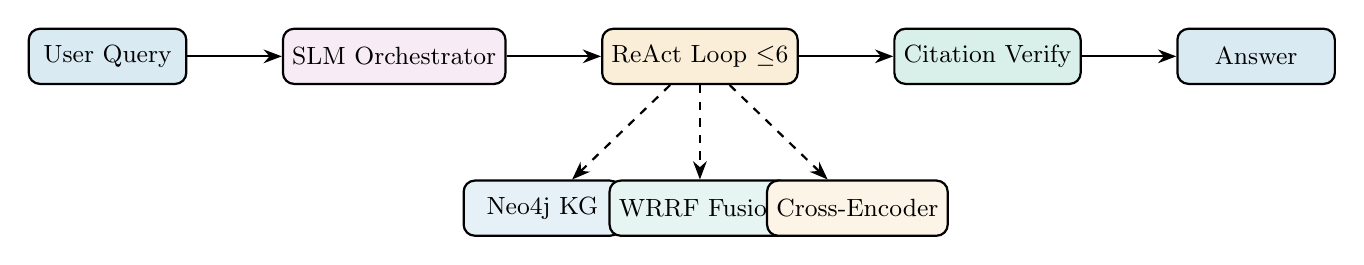
\begin{tikzpicture}[
  box/.style={draw, rounded corners, minimum width=2cm, minimum height=0.7cm, font=\small, thick},
  arr/.style={-{Stealth}, thick}
]
  \node[box, fill=positive!15] (query) {User Query};
  \node[box, fill=cbPurple!15, right=1.2cm of query] (slm) {SLM Orchestrator};
  \node[box, fill=negative!15, right=1.2cm of slm] (react) {ReAct Loop $\leq$6};
  \node[box, fill=emphasis!15, right=1.2cm of react] (cite) {Citation Verify};
  \node[box, fill=positive!15, right=1.2cm of cite] (ans) {Answer};

  \draw[arr] (query) -- (slm);
  \draw[arr] (slm) -- (react);
  \draw[arr] (react) -- (cite);
  \draw[arr] (cite) -- (ans);

  \node[box, fill=positive!10, below=1.2cm of react, xshift=-2cm] (neo4j) {Neo4j KG};
  \node[box, fill=emphasis!10, below=1.2cm of react] (vec) {WRRF Fusion};
  \node[box, fill=negative!10, below=1.2cm of react, xshift=2cm] (rerank) {Cross-Encoder};

  \draw[arr, dashed] (react) -- (neo4j);
  \draw[arr, dashed] (react) -- (vec);
  \draw[arr, dashed] (react) -- (rerank);
\end{tikzpicture}
}
\end{center}
\vspace{0.3em}
\begin{itemize}
  \item \textbf{Fully local} --- no external API calls; 16GB RAM, 8GB VRAM (RTX 3060/4060)
  \item \textbf{Model:} Qwen2.5-7B-Instruct, 4-bit NF4 ($\sim$5.5GB VRAM)
  \item \textbf{Reranker:} BAAI/bge-reranker-v2-m3 (multilingual cross-encoder)
\end{itemize}
\end{frame}

% SLIDE 8: Knowledge Graph
\begin{frame}{Knowledge Graph Construction}
\begin{columns}[T]
\column{0.50\textwidth}
\textbf{Typed Schema}\\[4pt]
{\small\ttfamily
(:Page) -[:HAS\_CHUNK]-> (:Chunk)\\
(:Chunk)-[:MENTIONS\_PERSON]->(:Person)\\
(:Chunk)-[:MENTIONS\_ORG]->(:Organization)\\
(:Chunk)-[:MENTIONS\_LOC]->(:Location)\\
(:Chunk)-[:MENTIONS\_WORK]->(:Work)\\
(:Page) -[:LINKS\_TO]-> (:Page)
}
\vspace{0.5em}

\textbf{Current scale:} 998 pages, 19K chunks, 3.3K entities

\column{0.45\textwidth}
\textbf{6 Pluggable NER Backends}
\begin{itemize}
  \item \textbf{Simple} --- regex + keyword classification
  \item \textbf{Underthesea} --- BIO tagging, offline
  \item \textbf{PhoNLP} --- VnCoreNLP + PhoNLP
  \item \textbf{PhoBERT} --- transformer pipeline
  \item \textbf{ViDeBERTa} --- electra-base NER
  \item \textbf{Wikilink} --- hyperlink extraction (best for bulk, Typed F1=46.9\%)
\end{itemize}
\vspace{0.3em}
All backends $\rightarrow$ \texttt{(name, type)} tuples $\rightarrow$ typed graph labels
\end{columns}
\end{frame}

% SLIDE 9: Text2Cypher
\begin{frame}{Text2Cypher Translation Pipeline}
\begin{center}
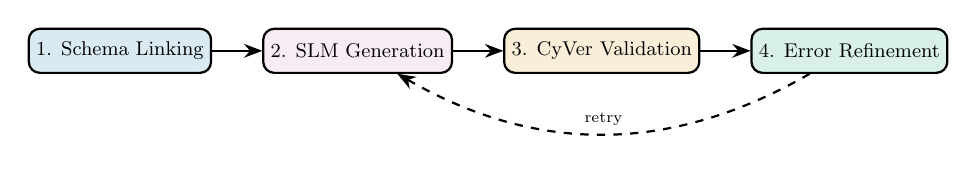
\begin{tikzpicture}[
  box/.style={draw, rounded corners, minimum width=2.8cm, minimum height=0.7cm, font=\small, thick},
  arr/.style={-{Stealth}, thick},
  scale=0.8, transform shape
]
  \node[box, fill=positive!15] (schema) {1. Schema Linking};
  \node[box, fill=cbPurple!15, right=0.8cm of schema] (gen) {2. SLM Generation};
  \node[box, fill=negative!15, right=0.8cm of gen] (val) {3. CyVer Validation};
  \node[box, fill=emphasis!15, right=0.8cm of val] (ref) {4. Error Refinement};

  \draw[arr] (schema) -- (gen);
  \draw[arr] (gen) -- (val);
  \draw[arr] (val) -- (ref);
  \draw[arr, dashed, bend left=30] (ref) to node[above, font=\scriptsize] {retry} (gen);
\end{tikzpicture}
\end{center}
\vspace{0.3em}
\vspace{0.3em}
\textbf{Example:} ``Tác phẩm `Tắt đèn' được sáng tác bởi nhà văn sinh năm bao nhiêu?''
\begin{exampleblock}{2-hop Vietnamese $\rightarrow$ Cypher}
{\ttfamily\small MATCH (tp:TacPham \{ten: "Tat den"\})<-[:SANG\_TAC]-(nv:NhaVan)\\
RETURN nv.nam\_sinh}
\end{exampleblock}
\small Inspired by CyVerACT (Androna et al., 2026) and Ozsoy et al. (2025, 2026)
\end{frame}

% SLIDE 10: Retrieval
\begin{frame}{Hybrid Retrieval with Cross-Encoder Reranking}
\begin{enumerate}
  \item \textbf{Schema Linking} --- BM25/TF-IDF prunes KG schema to relevant labels/relations
  \item \textbf{Cypher Generation} --- SLM produces read-only Cypher from query + pruned schema
  \item \textbf{Deterministic Validation} --- syntax check, write-keyword blocklist, alias verification
  \item \textbf{Hybrid Fallback} --- on invalid Cypher $\rightarrow$ BM25 + dense vector retrieval
  \item \textbf{Cross-Encoder Reranking} --- BAAI/bge-reranker-v2-m3 scores top-$k$
\end{enumerate}
\vspace{0.5em}
\begin{columns}[T]
\column{0.48\textwidth}
\begin{alertblock}{Why Hybrid?}
Graph-only degrades under KG sparsity (HybridRAG, 2026). Text fallback ensures coverage.
\end{alertblock}
\column{0.48\textwidth}
\begin{exampleblock}{Reranking Impact}
Cross-encoder reranking: \pos{+15.5\%} accuracy (literature benchmark)
\end{exampleblock}
\end{columns}
\end{frame}

% SLIDE 11: ReAct Agent
\begin{frame}{Tool-Constrained ReAct Agent}
\begin{columns}[T]
\column{0.48\textwidth}
\textbf{6 Deterministic Tools}
\begin{itemize}
  \item \texttt{kg\_schema()} --- cached JSON schema
  \item \texttt{kg\_query(cypher)} --- execute \& return rows/errors
  \item \texttt{text\_search(q, k)} --- hybrid BM25 + dense
  \item \texttt{get\_passage(id)} --- raw paragraph text
  \item \texttt{entity\_neighborhood(e)} --- 1-hop subgraph
  \item \texttt{path\_search(a, b)} --- shortest path
\end{itemize}

\column{0.48\textwidth}
\textbf{Agent Loop (pseudocode)}\\[3pt]
{\small\ttfamily
for i in 1..6:\\
\quad thought = SLM(obs)\\
\quad action = parse\_tool(thought)\\
\quad obs = execute(action)\\
\quad if sufficient(obs): break\\
answer = cite(obs, passage\_ids)
}
\end{columns}
\vspace{0.4em}
\small Sufficiency gating: empty KG $\rightarrow$ text\_search or abstain. Aligned with ReflectiveRAG, C2RAG.
\end{frame}

% SLIDE 12: Local SLM
\begin{frame}{Local SLM \& Fine-tuning Strategy}
\begin{columns}[T]
\column{0.48\textwidth}
\textbf{Runtime Configuration}
\vspace{4pt}
\begin{tabular}{ll}
\toprule
Parameter & Value \\
\midrule
Base Model & Qwen2.5-7B-Instruct \\
Quantization & 4-bit NF4 \\
Loading & Lazy, cached in memory \\
VRAM & $\sim$5.5GB \\
Interfaces & \texttt{generate()} + \texttt{chat()} \\
\bottomrule
\end{tabular}

\column{0.48\textwidth}
\textbf{Fine-tuning Plan}
\begin{itemize}
  \item \textbf{QLoRA} --- NF4, double quant, LoRA rank 32, all linear layers, 10--15K pairs
  \item \textbf{DPO Alignment} --- JSON tool-call compliance, schema correctness
  \item \textbf{Target:} $>$95\% executable Cypher
\end{itemize}
\vspace{0.3em}
\small Refs: QLoRA (Dettmers, 2023), DPO (Rafailov, 2023)
\end{columns}
\end{frame}

% SLIDE 13: Data Sources
\begin{frame}{Data Sources: ViQuAD 2.0 + ViWiki-MHR}
\begin{columns}[T]
\column{0.48\textwidth}
\begin{alertblock}{UIT-ViQuAD 2.0 (External)}
\begin{itemize}
  \item \textbf{39.5K} QA pairs, 174 Wikipedia articles
  \item Standard Vietnamese MRC benchmark (peer-reviewed)
  \item $\sim$12K unanswerable questions (SQuAD 2.0 style)
\end{itemize}
\end{alertblock}

\column{0.48\textwidth}
\begin{exampleblock}{ViWiki-MHR (Ours, CC-BY-SA)}
\begin{itemize}
  \item $\sim$36K multi-hop QA, 6 reasoning types
  \item Broken-link adversarial unanswerables (first VN)
  \item Gold passage IDs + executable Cypher queries
\end{itemize}
\end{exampleblock}
\end{columns}
\vspace{0.3em}
\begin{center}
\small
\begin{tabular}{lrrl}
\toprule
\textbf{Component} & \textbf{Size} & \textbf{Hops} & \textbf{Source} \\
\midrule
Single-hop answerable & $\sim$23K & 1 & UIT-ViQuAD 2.0 \\
Single-hop unanswerable & $\sim$5K & 1 & ViQuAD 2.0 adversarial \\
Multi-hop answerable & $\sim$7K & 2--3 & KG walks + LLM rewrite \\
\HL{Adversarial multi-hop} & $\sim$1K & 2--3 & \HL{Broken-link (first VN)} \\
\bottomrule
\end{tabular}
\end{center}
\end{frame}

% SLIDE 14: Dataset Generation
\begin{frame}{ViWiki-MHR Generation Pipeline}
\begin{center}
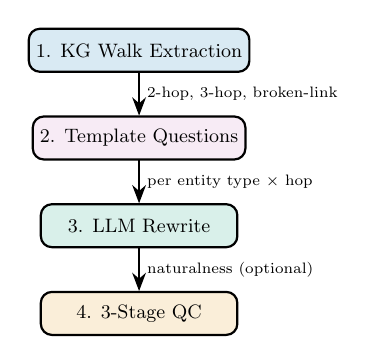
\begin{tikzpicture}[
  box/.style={draw, rounded corners, minimum width=3.2cm, minimum height=0.7cm, font=\small, thick},
  arr/.style={-{Stealth}, thick},
  scale=0.78, transform shape
]
  \node[box, fill=positive!15] (walk) {1. KG Walk Extraction};
  \node[box, fill=cbPurple!15, below=0.7cm of walk] (tmpl) {2. Template Questions};
  \node[box, fill=emphasis!15, below=0.7cm of tmpl] (rewrite) {3. LLM Rewrite};
  \node[box, fill=negative!15, below=0.7cm of rewrite] (qc) {4. 3-Stage QC};

  \draw[arr] (walk) -- node[right, font=\scriptsize] {2-hop, 3-hop, broken-link} (tmpl);
  \draw[arr] (tmpl) -- node[right, font=\scriptsize] {per entity type $\times$ hop} (rewrite);
  \draw[arr] (rewrite) -- node[right, font=\scriptsize] {naturalness (optional)} (qc);
\end{tikzpicture}
\end{center}
\vspace{0.3em}
\begin{columns}[T]
\column{0.48\textwidth}
\textbf{Reasoning taxonomy:} lookup, bridge, comparison, intersection, temporal, fan-out

\column{0.48\textwidth}
\textbf{QC:} well-formedness $\rightarrow$ grounding match $\rightarrow$ deduplication
\end{columns}
\vspace{0.3em}
\small Adversarial unanswerables inspired by BRINK (Zhou et al., 2026) --- break one link in valid KG path
\end{frame}

% SLIDE 15: ViQuAD2 Integration
\begin{frame}{ViQuAD 2.0 Integration Strategy}
\begin{columns}[T]
\column{0.48\textwidth}
\textbf{Integration Pipeline}
\begin{enumerate}
  \item HuggingFace load + format conversion
  \item Dedup (title + text hash)
  \item Ingest new passages into KG
  \item End-to-end eval (validation split)
\end{enumerate}

\column{0.48\textwidth}
\textbf{Why ViQuAD 2.0?}
\begin{itemize}
  \item \textbf{Objectivity} --- external, not self-generated
  \item \textbf{Comparability} --- CafeBERT: 77.5\% EM
  \item \textbf{Abstain testing} --- 12K impossible Qs
  \item \textbf{Generative gap} --- Token F1 measurement
\end{itemize}
\end{columns}
\vspace{0.5em}
\begin{block}{Results vs. Targets}
Token F1: 0.12 / 0.40 (needs QLoRA) \quad | \quad \pos{Context Hit Rate: 64.7\% $>$ 0.60} \quad | \quad Abstain: pending
\end{block}
\end{frame}

% SLIDE 16: Evaluation
\begin{frame}{Evaluation Framework \& Results}
\begin{columns}[T]
\column{0.45\textwidth}
\textbf{Metrics Suite}
\vspace{4pt}
\begin{tabular}{ll}
\toprule
Category & Metrics \\
\midrule
Retrieval & Hit Rate, MRR \\
Answer & Token F1, EM \\
Robustness & Abstain Accuracy \\
Efficiency & Avg Latency \\
Groundedness & Faithfulness \\
\bottomrule
\end{tabular}

\column{0.50\textwidth}
\textbf{Results (ViQuAD2, $n$=2652)}
\vspace{4pt}
\begin{tabular}{lr}
\toprule
Metric & Value \\
\midrule
\pos{Context Hit Rate} & \pos{64.7\%} \\
\pos{MRR} & \pos{0.450} \\
Token F1 & 0.120 \\
Avg Latency & 51 ms \\
\bottomrule
\end{tabular}
\end{columns}
\vspace{0.5em}
\begin{columns}[T]
\column{0.48\textwidth}
\begin{exampleblock}{Retrieval: Target Met}
Hit Rate 64.7\% $>$ 60\% target \checkmark\\
MRR 0.45 (rank 1--2 avg) \checkmark\\
Latency 51ms (well under 3s) \checkmark
\end{exampleblock}
\column{0.48\textwidth}
\begin{alertblock}{Generation: Needs Fine-tuning}
Token F1 = 0.12 (target 0.40)\\
\con{Root cause:} base SLM without task-specific fine-tuning; QLoRA planned
\end{alertblock}
\end{columns}
\end{frame}

% SLIDE 17: Demo
\begin{frame}{Live Demo}
\begin{exampleblock}{Sample Multi-hop Query}
\textbf{Q:} ``Ai sáng lập tổ chức có trụ sở tại Hà Nội?''\\[4pt]
\textbf{Reasoning:} Location(Hà Nội) $\leftarrow$[:TRỤ\_SỞ]--- Organization(X) $\leftarrow$[:SÁNG\_LẬP]--- Person(?)
\end{exampleblock}
\vspace{0.3em}
\textbf{Agent trace:}\\[3pt]
{\small\ttfamily
\{"tool": "kg\_query",\\
\ "cypher": "MATCH (l:Location\{name:'Hà Nội'\})<-[:TRU\_SO]-(o:Org)...",\\
\ "result": [\{"person": "Nguyễn Văn A", "passage\_id": "chunk-0042"\}],\\
\ "citations": ["chunk-0042"]\}
}
\end{frame}

% SLIDE 18: References
\begin{frame}{References}
\small
\begin{thebibliography}{9}
\bibitem{edge2024} Edge et al. (2024). From Local to Global: A Graph RAG Approach. \textit{Microsoft Research}.
\bibitem{cyveract} Androna et al. (2026). CyVerACT: Deterministic Cypher Validation. \textit{arXiv}.
\bibitem{ozsoy2025} Ozsoy et al. (2025). Text2Cypher: Schema-Conditioned Generation. \textit{Neo4j Research}.
\bibitem{dettmers2023} Dettmers et al. (2023). QLoRA: Efficient Finetuning of Quantized LLMs. \textit{NeurIPS}.
\bibitem{brink2026} Zhou et al. (2026). BRINK: Broken-Link Adversarial Unanswerables. \textit{arXiv}.
\bibitem{hisgraphrag} Nguyen et al. (2025). HisGraphRAG. \textit{PACLIC}.
\bibitem{viquad2} Nguyen et al. (2022). UIT-ViQuAD 2.0. \textit{UIT-NLP}.
\bibitem{liu2024} Liu et al. (2024). Lost in the Middle: How LLMs Use Long Contexts. \textit{TACL}.
\bibitem{reflectiverag} Verma et al. (2026). ReflectiveRAG: Sufficiency-Aware Retrieval. \textit{arXiv}.
\bibitem{hybridrag} Choudhary et al. (2026). HybridRAG: KG-Augmented Retrieval. \textit{arXiv}.
\end{thebibliography}
\end{frame}

% SLIDE 19: Q&A
\begin{frame}{Conclusion \& Future Work}
\begin{columns}[T]
\column{0.48\textwidth}
\begin{exampleblock}{Achieved}
\begin{itemize}
  \item End-to-end local GraphRAG (16GB RAM, 8GB VRAM)
  \item Typed Vietnamese KG (6 NER backends)
  \item ReAct agent + 6 tools + citation tracking
  \item WRRF hybrid retrieval (64.7\% hit rate)
  \item ViQuAD2 integration + multi-metric eval
\end{itemize}
\end{exampleblock}

\column{0.48\textwidth}
\begin{alertblock}{Future Directions}
\begin{itemize}
  \item QLoRA fine-tuning (Token F1: 0.12 $\rightarrow$ 0.40+)
  \item DPO alignment (tool compliance)
  \item Scale to 5000+ pages (full ViWiki)
  \item Abstain accuracy evaluation
  \item Multi-trajectory voting optimization
\end{itemize}
\end{alertblock}
\end{columns}
\end{frame}

\begin{frame}[plain]
\begin{center}
\vspace{2cm}
{\Huge \textbf{Thank You}}\\[1em]
{\Large Questions \& Discussion}\\[2em]
{\normalsize Vietnamese GraphRAG over Wikipedia + Neo4j}\\[0.5em]
{\small \textcolor{neutral}{Local-first $\cdot$ Multi-hop $\cdot$ Citation-grounded}}
\end{center}
\end{frame}

% BACKUP SLIDES
\appendix

\begin{frame}{Naive RAG vs. GraphRAG vs. Ours}
\vspace{4pt}
\begin{center}
\small
\begin{tabular}{llll}
\toprule
\textbf{Feature} & \textbf{Naive RAG} & \textbf{GraphRAG} & \textbf{Ours} \\
\midrule
Data repr. & Flat chunks & Graph + communities & Typed KG + text \\
Multi-hop & Poor & Excellent & Excellent + hybrid \\
Context & Large (raw) & Small (sub-graphs) & Small (Cypher) \\
Hallucination & None & Structural & CyVer + citations \\
Cost & Low & High (Leiden) & Medium (consumer) \\
\bottomrule
\end{tabular}
\end{center}
\end{frame}

\begin{frame}{Broken-Link Adversarial Construction}
\begin{exampleblock}{Valid vs. Broken Path}
\textbf{Valid:} (Ngô Tất Tố) ---[:SÁNG\_TÁC]$\rightarrow$ (Tắt đèn) ---[:BỐ\_CẢNH]$\rightarrow$ (Cẩm Giàng)\\[4pt]
\textbf{Broken:} (Ngô Tất Tố) ---[:SÁNG\_TÁC]$\rightarrow$ (Tắt đèn) ---[:BỐ\_CẢNH]$\rightarrow$ \con{[Fabricated: Hải Phòng]}
\end{exampleblock}
\vspace{0.3em}
\begin{itemize}
  \item Surface question coherent up to hop 2, fails at hop 3
  \item Forces agent to verify each path step programmatically
  \item System must output ``I don't know'' if link fails
  \item \HL{First Vietnamese benchmark} for multi-hop unanswerability
\end{itemize}
\end{frame}

\begin{frame}{QLoRA Training Configuration}
\vspace{4pt}
\begin{center}
\begin{tabular}{ll}
\toprule
\textbf{Parameter} & \textbf{Value} \\
\midrule
Bits & 4-bit NormalFloat (NF4) \\
Double Quantization & Enabled \\
Target Modules & All linear (q, k, v, o, gate, up, down) \\
LoRA Rank ($r$) & 32 \\
LoRA Alpha ($\alpha$) & 64 \\
Optimizer & Paged AdamW \\
Training Data & 10--15K Text2Cypher pairs \\
Evaluation & 500 human-verified held-out pairs \\
\bottomrule
\end{tabular}
\end{center}
\vspace{0.3em}
\textbf{Task 1:} Vietnamese Text2Cypher (primary)\\
\textbf{Task 2:} Agent action format conformance (secondary)
\end{frame}

\end{document}
